\subsection{Sick Dataset}
\label{sec:sick-data}
% B owns this subsection: UCI provenance, label meaning, missingness, and preprocessing.

The \textit{sick} dataset belongs to the UCI Thyroid Disease repository
(ID 102, DOI 10.24432/C5D010), with original data donated by the Garavan
Institute (1986) and redistributed under CC BY 4.0; we use the Weka-packed
variant (accepted by the course brief). The ``7,200 instances / 5
features'' on the UCI landing page describes the whole thyroid
repository, not this subset. The actual dataset contains
\textbf{3,772 instances $\times$ 30 attributes} (23 nominal, 7 numeric,
including the class). The class is severely imbalanced: 3,541
\textit{negative} versus 231 \textit{sick-euthyroid}, i.e.\ 6.1\%
positives (94:6); we treat \textit{sick} as the positive class
throughout. Two semantic notes we keep strict in wording:
\textit{sick-euthyroid} denotes a euthyroid patient whose
thyroid-related blood tests are abnormal --- notably low T3 --- while the
thyroid gland itself is not diseased; the pattern usually reflects severe
non-thyroidal illness such as chronic renal failure, diabetes or anaemia
(UCI \texttt{thyroid.theory}). It is \emph{not} hypothyroidism, which is a
separate sub-dataset. \textit{negative} means no thyroid abnormality
detected in this screening, not ``perfectly healthy''. 61
duplicate rows exist in the official distribution; we keep them to remain
consistent with the official instance count and disclose them as a
data-quality issue.

\subsubsection{Missing-value audit}
In total 6,064 cells (5.4\%) are missing, coded as ``?''. The audit
revealed a clean \emph{measurement mechanism}: every laboratory test
appears as a pair --- a \texttt{*\_measured} flag and the value itself ---
and whenever the flag reads \texttt{f} (test not performed), the paired
value is missing \emph{by design}. Across all six lab pairs the
consistency check found \textbf{zero anomalies}: the data is incomplete
but internally consistent. The extreme case is \textbf{TBG, 100\% missing
in all 3,772 rows} (its flag reads \texttt{f} in every row). After
removing TBG and its constant flag, 1,129 rows
(29.9\%) still carry at least one missing value
(Figs.~\ref{fig:sick-dist}--\ref{fig:sick-missing}).

\subsubsection{Handling decisions}
Three decisions follow directly from the audit, in the same
decision-plus-ablation style as the credit-g preprocessing above:

\begin{enumerate}
\item \textbf{Remove} TBG and its constant flag. A column with zero
observations cannot be imputed without fabricating data; column removal
involves no statistics and is leakage-free.
\item \textbf{Impute} the remaining columns \emph{inside} the imblearn
pipeline (numeric by mean, nominal by mode), so imputation statistics
are fitted on training folds only, alongside encoding, scaling and
SMOTE.
\item \textbf{Keep} the 61 duplicate rows, staying consistent with the
official instance count (disclosed above as a data-quality note).
\end{enumerate}

Decision~2 was validated by the same style of controlled ablation as the
credit-g encoding choice (Table~\ref{tab:a_encoding}): one decision
tree, one locked protocol, three missing-value treatments
(Table~\ref{tab:b_imputation}). Dropping incomplete rows discards
1{,}129 patients --- 19 of them positive --- for an F1 difference within
one standard deviation and the lowest AUC, and the two cohorts are not
even the same patients. Treating ``missing'' as its own category (an
option here because scikit-learn trees, unlike Weka's J48, reject
\texttt{NaN} values) performs no better. Fold-internal imputation keeps
all 3{,}772 instances and attains the best AUC, and was therefore locked
in the preprocessing spec (full fold-level results archived in
\texttt{results/b4\_missing\_comparison.csv}). The contrast with
credit-g is instructive: there the ablation \emph{changed} the decision
(which encoding to use), whereas here it \emph{confirmed} the default
--- the informative question on sick is not which treatment wins on F1,
but what deleting rows would cost.

\begin{table}[htbp]
\centering
\caption{Missing-value treatments on sick (decision tree, entropy,
\texttt{ccp\_alpha}=0.01; cv10, mean$\pm$std, ddof$=0$; positive
= sick-euthyroid).}
\label{tab:b_imputation}
\begin{tabular}{lccc}
\toprule
Treatment & Rows & F1 & ROC-AUC \\
\midrule
Fold-internal imputation (adopted) & 3{,}772 & 0.830$\pm$0.049 & \textbf{0.974} \\
Drop incomplete rows & 2{,}643 & 0.843$\pm$0.069 & 0.964 \\
``Missing'' as explicit category & 3{,}772 & 0.828$\pm$0.044 & 0.965 \\
\bottomrule
\end{tabular}
\end{table}
Finally, among the four base classifiers the random forest is the only
one whose precision is preserved under SMOTE (0.94$\to$0.91, vs.\
0.95$\to$0.60 for a single tree); Section~\ref{sec:results} sharpens this
account with the ensemble study, where AdaBoost shares the property and
plain bagging does not.

\begin{figure}[htbp]
\centering
\begin{minipage}{0.48\linewidth}
  \centering
  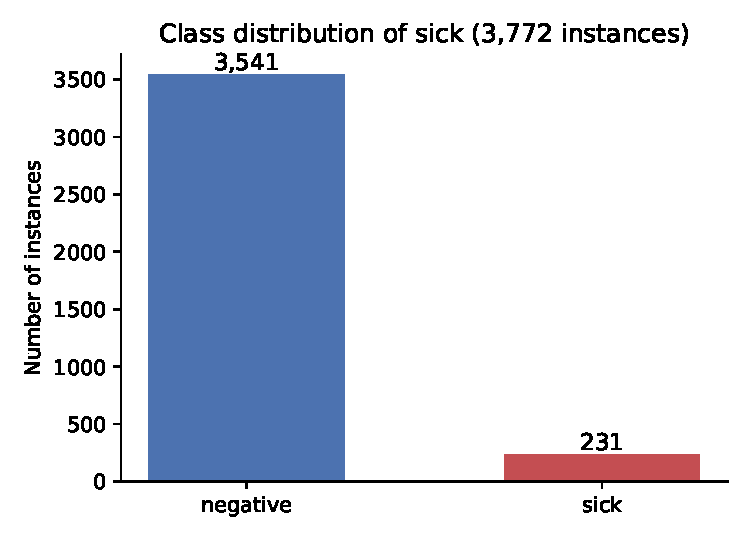
\includegraphics[width=\linewidth]{figures/fig_b_class.pdf}
  \caption{Class distribution of sick (3,541:231, 6.1\% positives; cv10,
  positive = sick-euthyroid).}\label{fig:sick-dist}
\end{minipage}\hfill
\begin{minipage}{0.48\linewidth}
  \centering
  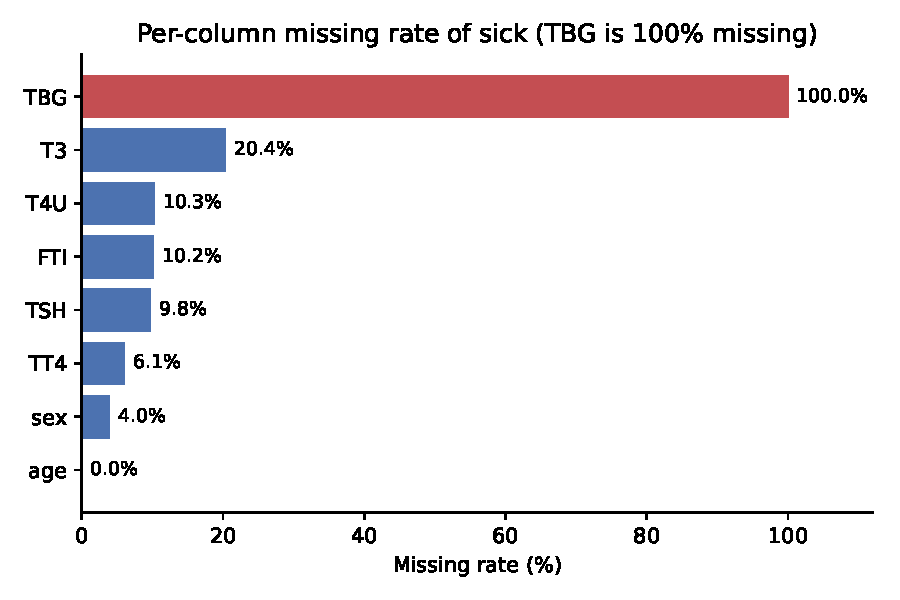
\includegraphics[width=\linewidth]{figures/fig_b_missing.pdf}
  \caption{Per-column missing rate of sick; TBG (red) is 100\% missing
  and removed rather than imputed.}\label{fig:sick-missing}
\end{minipage}
\end{figure}

\begin{figure}[htbp]
\centering
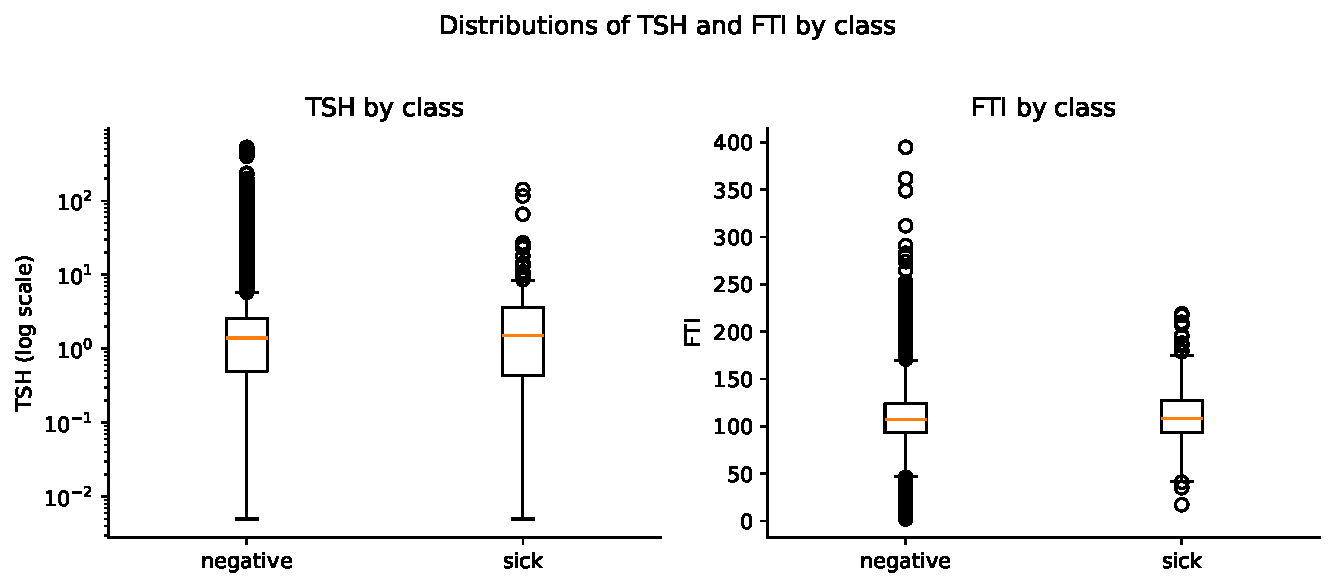
\includegraphics[width=0.62\linewidth]{figures/fig_b_box.pdf}
\caption{TSH (log scale) and FTI by class (raw data): heavy class overlap
(median TSH 1.4 vs.\ 1.5; FTI 107 vs.\ 108) shows no single lab value
separates the classes, motivating multivariate models.}\label{fig:sick-box}
\end{figure}
